\documentclass[11pt]{article}
\usepackage[margin=1in]{geometry}
\usepackage{amsmath,amssymb}
\usepackage{graphicx}
\usepackage{booktabs}
\usepackage[colorlinks=true,linkcolor=blue,citecolor=blue,urlcolor=blue]{hyperref}
\usepackage{natbib}
\usepackage{caption}

\graphicspath{{figures/}{../figures/}}

\title{Implied-volatility asymptotics at a\\
$C^{2}$ ATM local-volatility knot}
\author{Martial Ren\\\texttt{martialren@gmail.com}}
\date{\today}

\newcommand{\sloc}{\sigma_{\mathrm{loc}}}
\newcommand{\siv}{\sigma_{\mathrm{IV}}}
\newcommand{\ivhm}{\mathrm{iv}_{\mathrm{hm}}}
\newcommand{\Hev}{\mathrm{H}}

\begin{document}
\maketitle

\begin{abstract}
The standard practice is to parametrise the \emph{local} volatility
$\sloc$ and push it to implied volatility through the leading-order
Berestycki--Busca--Florent (BBF) inverse-harmonic-mean map. BBF can
calibrate essentially any market smile; its weakness is not fit but
consistency --- being only leading order, the implied vol it returns is
not the model's true Dupire implied vol, so a surface that matches quotes
can still carry small static-arbitrage inconsistencies. The
Henry-Labord\`ere $\sigma_1 T$ correction (PHL1) is the next order and
much closer to the true Dupire implied vol; moving from BBF to PHL1 buys
\emph{arbitrage reassurance}, not extra calibration reach. But PHL1 on a
single smooth cubic is rigid, and admitting a knot --- the natural way to
recover flexibility --- breaks it: a piecewise-cubic $\sloc$ is only $C^2$
at its knots (the cubic coefficient $\gamma=\sloc'''$ jumps), while the
$\sigma_1$ expansion is derived assuming $C^3$, leaving a localised
residual at the knot. We close that residual in the practically relevant
case --- a knot pinned exactly at-the-money --- in closed form: at first
order in the coefficient jump it is the first-order Duhamel kernel
$K_1(x,0)$ --- a one-dimensional bridge integral with peak
$3\sqrt{2\pi}/128$ and no fitted constants. This makes ``piecewise-cubic with an at-the-money knot, mapped
through PHL1'' a usable parametrisation that keeps PHL1's arbitrage
reassurance while regaining calibration flexibility. The at-the-money
restriction is essential, not cosmetic: off-the-money the same
construction needs an unbounded-polynomial truncation, which the $w=0$
case removes. We validate against the Dupire PDE on parameters calibrated
from real SPXW surfaces.
\end{abstract}

\section{Introduction}

When calibrating a volatility surface, practitioners fit a parametric
\emph{local} volatility (for the monotonicity and regularity an optimiser
needs) and map it to implied volatility with the leading-order BBF
inverse-harmonic-mean formula. BBF is flexible enough to calibrate
essentially any smile, so the motivation for going further is not fit.
It is \emph{arbitrage reassurance}: BBF is only leading order, so the
implied vol it returns is not the local-vol model's true Dupire implied
vol, and a quote-matching surface can still violate static no-arbitrage
(butterfly, calendar) at the sub-basis-point level that an
arbitrage-sensitive consumer cannot tolerate. The next-order PHL1 map is
much closer to the true Dupire implied vol and removes most of that
inconsistency.

The price of PHL1 is rigidity: a single smooth cubic mapped through PHL1
spans far fewer smile shapes than the loose BBF fit. The natural fix ---
a piecewise-cubic $\sloc$ with a knot --- fails, because PHL1's $\sigma_1$
heat-kernel term is derived for $C^3$ surfaces whereas a piecewise cubic
is only $C^2$ at a knot; the result is a localised implied-vol residual
at the knot strike (BBF, a harmonic-mean integral, is insensitive to it).
This paper removes that residual in closed form for a knot pinned
at-the-money, so the combination ``piecewise-cubic-with-ATM-knot $+$
PHL1'' becomes usable: it keeps PHL1's arbitrage reassurance while
recovering the calibration flexibility a smooth cubic lacks. The
correction is a parameter-free first-order Duhamel kernel; the
at-the-money restriction is what keeps it bounded. The same
derivation settles the open question Costeanu and Pirjol
\citep{costeanuPirjol2011} raise after their eq.~(5.25): whether the
absence of $T^{3/2}, T^{5/2}, \ldots$ non-analytic terms in their
$C^{0}$ symmetric model is general or model-specific --- it is the
latter, with a $T^{3/2}$ term and a clean universal coefficient
appearing as soon as the knot regularity is raised to $C^{2}$. The
remainder derives the correction and validates it against the Dupire
forward PDE \citep{dupire1994}.

\section{Related work}

The map from a parametric local-vol surface to implied vol through a
small-time asymptotic is one strand of a wider literature on parametric
volatility surfaces. The direct predecessor for the knot-residual
question, the broader asymptotic-map literature, and the orthogonal
parametric and arbitrage-framing literatures are taken in turn.

\paragraph{Direct prior art and open question.} The closest
predecessor is Costeanu--Pirjol \citep{costeanuPirjol2011}, who set up
the same Duhamel-perturbation framework for the analogous problem one
regularity class harsher: a $C^{0}$ local vol with a jump in
$\sigma'_{\mathrm{loc}}$ at the forward, in \emph{normal} (Bachelier)
implied vol. They prove that the ATM normal IV picks up a
non-analytic $\sqrt{T}$ term with universal coefficient
$\tfrac{1}{16}\sqrt{\pi/2}\approx 0.0784$ proportional to the jump,
and their Table~5.1 lists the powers of $T$ that can arise from each
order of perturbation in the same framework. After eq.~(5.25) they
note that their explicit symmetric-model solution contains only the
$\sqrt{T}$ non-analytic term, with no $T^{3/2}$, $T^{5/2}$, \ldots,
and leave open whether that absence is a general feature or specific
to their piecewise-linear model. The contribution here settles the
question: it is model-specific. A $C^{2}$ piecewise-cubic local vol
with the knot at the forward (the natural smoothness of a
piecewise-cubic calibrator, where only $\sigma'''_{\mathrm{loc}}
=\gamma$ jumps) produces a $T^{3/2}$ non-analytic term in
\emph{log-normal} Black IV --- the $T^{3/2}$ slot of their Table~5.1
row $n=1$, one column past the $\sqrt{T}$ slot they filled --- with
universal coefficient $3\sqrt{2\pi}/128\approx 0.0588$, the $C^{2}$
companion to their $C^{0}$ constant within the same Duhamel
lineage. The kernel $K_1(x,0)$ derived in Section~3 is the
corresponding first-order Duhamel kernel for the local-volatility
perturbation; in its bridge form it is a one-dimensional integral over
$\lambda\in[0,1]$ whose integrand is the conditional expectation of the
source along a standard Brownian bridge.

\paragraph{Higher-order LV-to-IV asymptotics.} The PHL1/GHLOW2 line
derives from the heat-kernel expansion of the call-price PDE: BBF
\citep{berestycki2002} is leading order (the same authors extended the
heat-kernel approach to stochastic volatility in
\citep{berestycki2004sv}), Henry-Labord\`ere \citep{henrylabordere2008}
adds $\sigma_1$, and Gatheral, Hsu, Laurence, Ouyang and Wang
\citep{gatheral2012} add $\sigma_2$ (Paulot
\citep{paulot2009} derives the second-order expansion
on the stochastic-volatility side, with SABR as the worked example). A parallel
methodology, due to Pagliarani--Pascucci \citep{pagliarani2012} and
extended to local--stochastic models by Lorig--Pagliarani--Pascucci
\citep{lorig2017}, derives implied-vol
expansions by Taylor-expanding the diffusion coefficients about a
point where they are assumed smooth; the knot case here is non-smooth
at the natural expansion point and lies outside that scope. A further
parallel route due to Medvedev and Scaillet
\citep{medvedevScaillet2007} writes the implied-vol PDE in
moneyness-degree $\theta=k/(\sigma\sqrt T)$ and solves an ODE in
$\theta$ at each order in $\sqrt T$; the polynomial-in-$\theta$
solution class assumed there is broken by the non-smooth forcing a
$C^2$ knot would inject into the same ODE. A
quadrature-based alternative due to Guyon and Henry-Labord\`ere
\citep{guyonHenryLabordere2010} sidesteps the smoothness assumption
entirely --- their heat-kernel estimator writes $\siv^2$ as a
weighted space--time average of $\sloc^2$ evaluated at quadrature
points, so a $C^2$ knot is handled by construction with no
correction term --- at the cost of a 2D quadrature per strike and
no closed-form $\siv(k;\theta)$ for an optimiser to differentiate.
De~Marco's harmonic-mean characterisation \citep{demarco2021} pins
what the leading-order map is approximating, and hence what the
next-order gap (the object PHL1c closes) actually is.

\paragraph{Direct implied-vol parametrisations.} The other side of the
design choice is to parametrise the implied-vol surface directly. SABR
\citep{hagan2002} fits a leading-order asymptotic of a stochastic-vol
model. SVI \citep{gatheral2004svi} and its arbitrage-free refinement
SSVI \citep{gatheralJacquier2014} drop the dynamic model and write the
smile itself as a parametric form, then constrain the parameters to
enforce static no-arbitrage. Andreasen--Huge \citep{andreasenHuge2011}
fits a piecewise-constant local vol in one implicit-Euler step of the
Dupire PDE; the resulting prices are arbitrage-free in the sense of the
discretised scheme, with as many vol pieces as quotes. This is a
different design point from ours: the local vol is piecewise-constant
so it carries no smooth parametric derivatives for an optimiser to
follow, the calibration carries a numerical scheme inside it (there
is no closed-form $\siv(k;\theta)$), and ``arbitrage-free'' is the
one-step finite-difference notion rather than the continuous Dupire
model's. Itkin and Lipton \citep{itkinLipton2018} sharpen the
analytical thread of this family by fitting a piecewise-linear local
variance via Laplace transform in time and Kummer hypergeometric
functions in space, which removes the FD-discretisation step but
keeps the piecewise low-order parametric structure and the lack of a
closed-form $\siv(k;\theta)$. The
parametric-LV-through-PHL1 route trades that for a closed-form
asymptotic on the local-vol side, with arbitrage reassurance carried
by PHL1's tightness against the true Dupire implied vol.

\paragraph{Static arbitrage and asymptotic constraints.}
``Arbitrage reassurance'' above is what Roper \citep{roper2010}
catalogues as static no-arbitrage on the IV surface (butterfly,
calendar). At the opposite end of the strike axis, Lee's moment formula
\citep{lee2004} gives the universal asymptotic bound on the deep-wing
slope of any arbitrage-free IV smile, and thereby on every map in the
family this paper works in. The contribution sits between the two: at
ATM, where Lee's tail bound is silent and the static-arbitrage
conditions reduce to a single local statement at $k=0$ --- and where the
$C^3$-regularity failure of a piecewise-cubic local vol is what PHL1
sees.

\section{Setup}

\paragraph{Units.} Two regimes throughout the paper. Anything displayed
--- the cubic definition below, figures, error tables --- is in
annualised \%. Anything inside an asymptotic-map formula --- BBF0,
$\sigma_1$, $\sigma_2$, the kernels $K_1$ / $K_1^{\mathrm{dir}}$ /
$K_1^{\mathrm{ext}}$, the knot correction --- is in total-vol units.
The scale factor introduced after eq.~\eqref{eq:perturb} converts at
the boundary; within either regime the symbols $\sigma,\beta,\alpha,
\gamma,\delta$ denote that regime's numerical values. This matches
practitioner convention: plotting is in annualised vols, numerical
methods are in total-vol.

Work in log-moneyness $k=\log(K/F)$, forward measure ($F=1$, $r=0$), single
maturity. The local volatility is time-homogeneous and cubic in
log-moneyness, in annualised \% units:
\begin{equation}
\sloc(k) = \sigma + \beta k + \alpha k^2 + \gamma k^3 .
\end{equation}
A knot at the money adds a one-sided jump $\delta$ in the cubic coefficient,
\begin{equation}
\sloc(k) = \sigma + \beta k + \alpha k^2 + \gamma k^3
           + \delta\,k^3\,\Hev(k) ,
\label{eq:perturb}
\end{equation}
with $\Hev$ the Heaviside step. Because $k^3$ and its first two derivatives
vanish at $k=0$, \eqref{eq:perturb} is $C^2$ at the knot; only $\sloc'''$
jumps by $\delta$. This is precisely the structure a piecewise-cubic
calibrator produces, with the knot moved to ATM.

We use the Black $T=1$ convention; $\mathrm{scale}=\sqrt{252/n}\cdot 100$
maps total vol to annualised \% for $n=\max(1,\mathrm{DTE})$ business
days. Each cubic coefficient is divided by $\mathrm{scale}$ when it
enters an asymptotic-map formula and multiplied back at the output, per
the Units convention above.

\paragraph{The asymptotic maps.} The leading-order BBF map
\citep{berestycki2002} is the inverse harmonic mean
\begin{equation}
\sigma_0(k)\equiv\ivhm(k)=k\Big/\!\int_0^k \frac{dy}{\sloc(y)},
\qquad \sigma_0(0)=\sloc(0),
\end{equation}
whose use as a smile parametrisation has practitioner precedent in Hagan
and Woodward \citep{haganWoodward1999}, who fit market smiles through an
equivalent constant-vol approximation; the structural properties of the
harmonic-mean representation itself are characterised in detail by
De~Marco \citep{demarco2021}.
The next-to-leading heat-kernel expansion of Henry-Labord\`ere
\citep{henrylabordere2008} adds a $\sigma_1 T$ term, giving
$\siv\approx\sigma_0+\sigma_1$. We use the explicit per-strike closed form of
that correction as stated by Gatheral, Hsu, Laurence, Ouyang and Wang
\citep[Thm.~2.4]{gatheral2012}, and keep the conventional label
\textbf{PHL1} for it:
\begin{equation}
\sigma_1(k)=\frac{\sigma_0(k)^3}{2k^2}
  \log\!\frac{\sqrt{\sloc(0)\,\sloc(k)}}{\sigma_0(k)} .
\label{eq:phl1}
\end{equation}
(Henry-Labord\`ere's own local-to-implied first-order result is the same
correction in the equivalent Hagan--Woodward \citep{haganWoodward1999}
midpoint form.) The GHLOW2
refinement adds a further $\sigma_2 T^2$ term from the same source
\citep{gatheral2012}. BBF0 is a harmonic mean of $\sloc$: a $C^2$ knot only
jumps $\sloc'''$, so the integrand $1/\sloc$ stays $C^2$ and $\sigma_0$ is
smooth across the knot --- BBF0 has no knot-specific error, only the generic
leading-order gap present everywhere. The $\sigma_1$ expansion underlying
PHL1 (and hence GHLOW2) is, by contrast, derived assuming $\sloc\in C^3$; at
a $C^2$-only knot it leaves a localised residual --- exactly the term this
note supplies.

\section{The at-the-money knot correction}

The implied-vol response to \eqref{eq:perturb} expands in the jump $\delta$
about the knotless case. At first order, in dimensionless strike
$x=k/\sigma$,
\begin{equation}
\delta\siv(k) \;=\; \delta\cdot\sigma^{3}\cdot K_1(x,0)
\;+\;O(\delta^2).
\label{eq:expansion}
\end{equation}

We call $K_1$ the \emph{first-order Duhamel kernel} for the
local-volatility perturbation: the first-order term of the Dyson series
for the perturbed call-price evolution against constant-$\sigma$ Black.
The bridge form derived below is that Duhamel integral after a
$\lambda=\tau/T$ rescaling exposes the conditional law of the
intermediate position as a standard Brownian bridge; the bridge framing
is bookkeeping for the small-$T$ scaling, not separate machinery.

\paragraph{Very simple derivation.}
First order in $\delta$, the source is $v(y)=2\sigma\,\delta\,y^3\Hev(y)$.
Inserting it once into the Duhamel expansion of the Dupire call price
against the constant-$\sigma$ Black heat kernel, the Black strike-gamma
identity cancels the explicit $\sigma$, and a Gaussian completion turns the
spatial integral into an expectation under a Brownian bridge pinned at
$(0,0)$ and $(k,T)$: writing $\lambda=t/T$, the bridge has
$y\sim\mathcal N(\lambda k,\;\sigma^2\lambda(1-\lambda))$. The remaining
$y$-integral against $y^3\Hev(y)$ is a truncated third moment of a normal,
\begin{equation}
f(\eta)=(\eta^3+3\eta)\,\Phi(\eta)+(\eta^2+2)\,\phi(\eta),
\end{equation}
with $\Phi,\phi$ the standard normal cdf/pdf. The $\sqrt\lambda$ from the
Gaussian completion cancels the $1/\sqrt t$ of the strike-gamma, the outer
time integral collapses to a clean bridge-time integral, and dividing by
the Black vega gives \eqref{eq:expansion} with
\begin{equation}
\boxed{\;K_1(x,0)=\int_0^1\big(\lambda(1-\lambda)\big)^{3/2}
   f\big(\eta(\lambda;x)\big)\,d\lambda,\qquad
   \eta(\lambda;x)=x\sqrt{\tfrac{\lambda}{1-\lambda}}.\;}
\label{eq:K1}
\end{equation}
At the knot centre $\eta\equiv0$, $f(0)=2/\sqrt{2\pi}$, and the integral is
a Beta function:
\begin{equation}
K_1(0,0)=\frac{2}{\sqrt{2\pi}}\,B\!\left(\tfrac52,\tfrac52\right)
=\frac{3\sqrt{2\pi}}{128}\approx 0.05875 .
\end{equation}

\paragraph{Why at-the-money.} The general knot at offset
$w=k_{\mathrm{knot}}/\sigma$ keeps a factor $\eta=[\lambda x-(1-\lambda)w]/
\sqrt{\lambda(1-\lambda)}$; the subtraction below then leaves a polynomial
that grows without bound and needs an ad-hoc truncation to stay finite.
Setting $w=0$ removes the $(1-\lambda)w$ term entirely and the correction is
bounded with no hack --- the reason this note restricts to the ATM knot.

\paragraph{Avoiding double counting.} PHL1 already moves under
\eqref{eq:perturb} through its own $\sigma_0$ and $\sigma_1$. Taylor-expanding
\eqref{eq:phl1} in $\delta$ at $w=0$ gives, for $x>0$,
$\sigma_0$ varies as $x^3/4$ and $\sigma_1$ as $x/4$ (both zero for $x\le0$).
Subtracting these so they are not counted twice yields the \emph{directed}
kernel, which decays on both sides:
\begin{equation}
K_1^{\mathrm{dir}}(x,0)=
\begin{cases}
K_1(x,0)-\dfrac{x^3}{4}-\dfrac{x}{4}, & x>0,\\[2ex]
K_1(x,0), & x\le 0.
\end{cases}
\label{eq:K1-dir}
\end{equation}
We will refer to \eqref{eq:K1-dir} as the \emph{universal} directed
kernel: it is a pure function of $x=k/\sigma$, identical for every
cubic. Section~\ref{sec:results} introduces a second, \emph{extended}
directed kernel that adds one $(\beta,\alpha,\gamma)$-parametric subtraction --- the
\emph{extension piece}, or just the \emph{extension} --- to absorb a
$\sigma_2$-only discontinuity that the universal kernel cannot reach.
The two kernels define our three closed-form knot corrections: PHL1c
(PHL1 baseline + universal kernel), GHLOW2c (GHLOW2 baseline +
universal kernel), and GHLOW2cc (GHLOW2 baseline + extended kernel
$=$ universal kernel $+$ extension).
\paragraph{The correction symbol.} Following the $\sigma_1, \sigma_2$
convention where each closed-form contribution to $\siv$ is a named
quantity, write
\begin{equation}
R^{(3, 1)}_{1}(x, w) \;\equiv\; \delta\cdot\sigma^{3}\cdot K_1^{\mathrm{dir}}(x, w),
\qquad
R^{(3, 1)}_{2}(x, w) \;\equiv\; \delta\cdot\sigma^{3}\cdot K_1^{\mathrm{ext}}(x, w),
\label{eq:R-def}
\end{equation}
with $(x, w) = (k/\sigma, k_{\mathrm{knot}}/\sigma)$ inherited from
$K_1$'s arguments, and $K_1^{\mathrm{ext}}$ the extended kernel
\eqref{eq:ghlow2-dir} of Section~\ref{sec:results}. The two
superscripts are the constants of this paper: $3$ is the
$\sigma_{\mathrm{loc}}'''$ jump level, and $1$ is the Duhamel-expansion
order (first order in $\delta$). The lone subscript $n$ is what varies
between the two corrections --- the baseline T-order whose
$\delta$-variations are subtracted from the bridge integral $K_1$ to
give the kernel. The ATM restriction $w=0$ is visible at every
callsite. Costeanu and Pirjol's universal coefficient
\citep{costeanuPirjol2011} sits in the same family at
$R^{(1, 1)}_{0}(0, 0)$.

The corrected PHL1 method, with PHL1 evaluated on the perturbed surface
so the cancellation is exact to first order, is
\begin{equation}
\siv^{\mathrm{PHL1c}}(k)=\siv^{\mathrm{PHL1}}(k)+R^{(3, 1)}_{1}(k/\sigma, 0).
\end{equation}
We use the suffix ``c'' (lower-case) throughout for ``one closed-form
knot-correction layer applied to this baseline'': PHL1c and GHLOW2c
each carry one such layer (the universal kernel), while GHLOW2cc
carries two (universal kernel + the extended subtraction), one $c$
per layer.
The bridge integral \eqref{eq:K1} is evaluated with a 32-point
Gauss--Legendre rule.

Table~\ref{tab:summary} summarises every method, kernel, and term
introduced above.

\begin{table}[h]
\centering
\begin{tabular}{llll}
\toprule
Name      & Definition                                              & Smooth order & Knot correction \\
\midrule
BBF0      & $\sigma_0$                                              & $T^{0}$ & --- \\
PHL1      & $\sigma_0 + \sigma_1$                                   & $T^{1}$ & --- \\
PHL1c     & $\sigma_0 + \sigma_1 + R^{(3, 1)}_{1}$                  & $T^{1}$ & $T^{3/2}$ \\
GHLOW2    & $\sigma_0 + \sigma_1 + \sigma_2$                        & $T^{2}$ & --- \\
GHLOW2c   & $\sigma_0 + \sigma_1 + R^{(3, 1)}_{1} + \sigma_2$       & $T^{2}$ & $T^{3/2}$ \\
GHLOW2cc  & $\sigma_0 + \sigma_1 + R^{(3, 1)}_{1} + \sigma_2 + (R^{(3, 1)}_{2} - R^{(3, 1)}_{1})$ & $T^{2}$ & $T^{3/2},\,T^{2}$ \\
\bottomrule
\end{tabular}
\caption{The six closed-form approximations to the Dupire IV. The ``c''
suffix counts correction layers stacked on a baseline: one $c$ per
layer. ``Smooth order'' is the heat-kernel-ladder accuracy in the
no-knot case; ``knot correction'' lists the orders at the knot the
corrections restore on top of the smooth baseline --- $T^{3/2}$ from
the universal kernel \eqref{eq:K1-dir} (the slope-kink term
$\sigma_1/\sigma_2$ miss at $C^{2}$), and additionally $T^{2}$ from the
extension piece \eqref{eq:extension} (the $\sigma_2(0)$ value jump
closed only by GHLOW2cc, on $k>0$).}
\label{tab:summary}
\end{table}

\section{Results}\label{sec:results}

Parameters come from real SPXW surfaces calibrated with a 20-parameter
piecewise-cubic local-vol model; we keep the centre cubic and (for the knot
case) the first-knot coefficient jump moved to ATM. The Dupire forward PDE
(Rannacher start then Crank--Nicolson) is the ground truth.

Figure~\ref{fig:happy}: a smooth monotone-skew smile (SPXW 2025-03-10
DTE~1, no knot). BBF0 sits $\sim$67~bps from the Dupire PDE across the
band while PHL1 and GHLOW2 close to a few bps. The bps gap is not the
objective in itself --- it is the measure of how far each map is from the
model's true Dupire implied vol, i.e.\ of the static-arbitrage slack PHL1
removes relative to BBF0.

\begin{figure}[!htbp]
\centering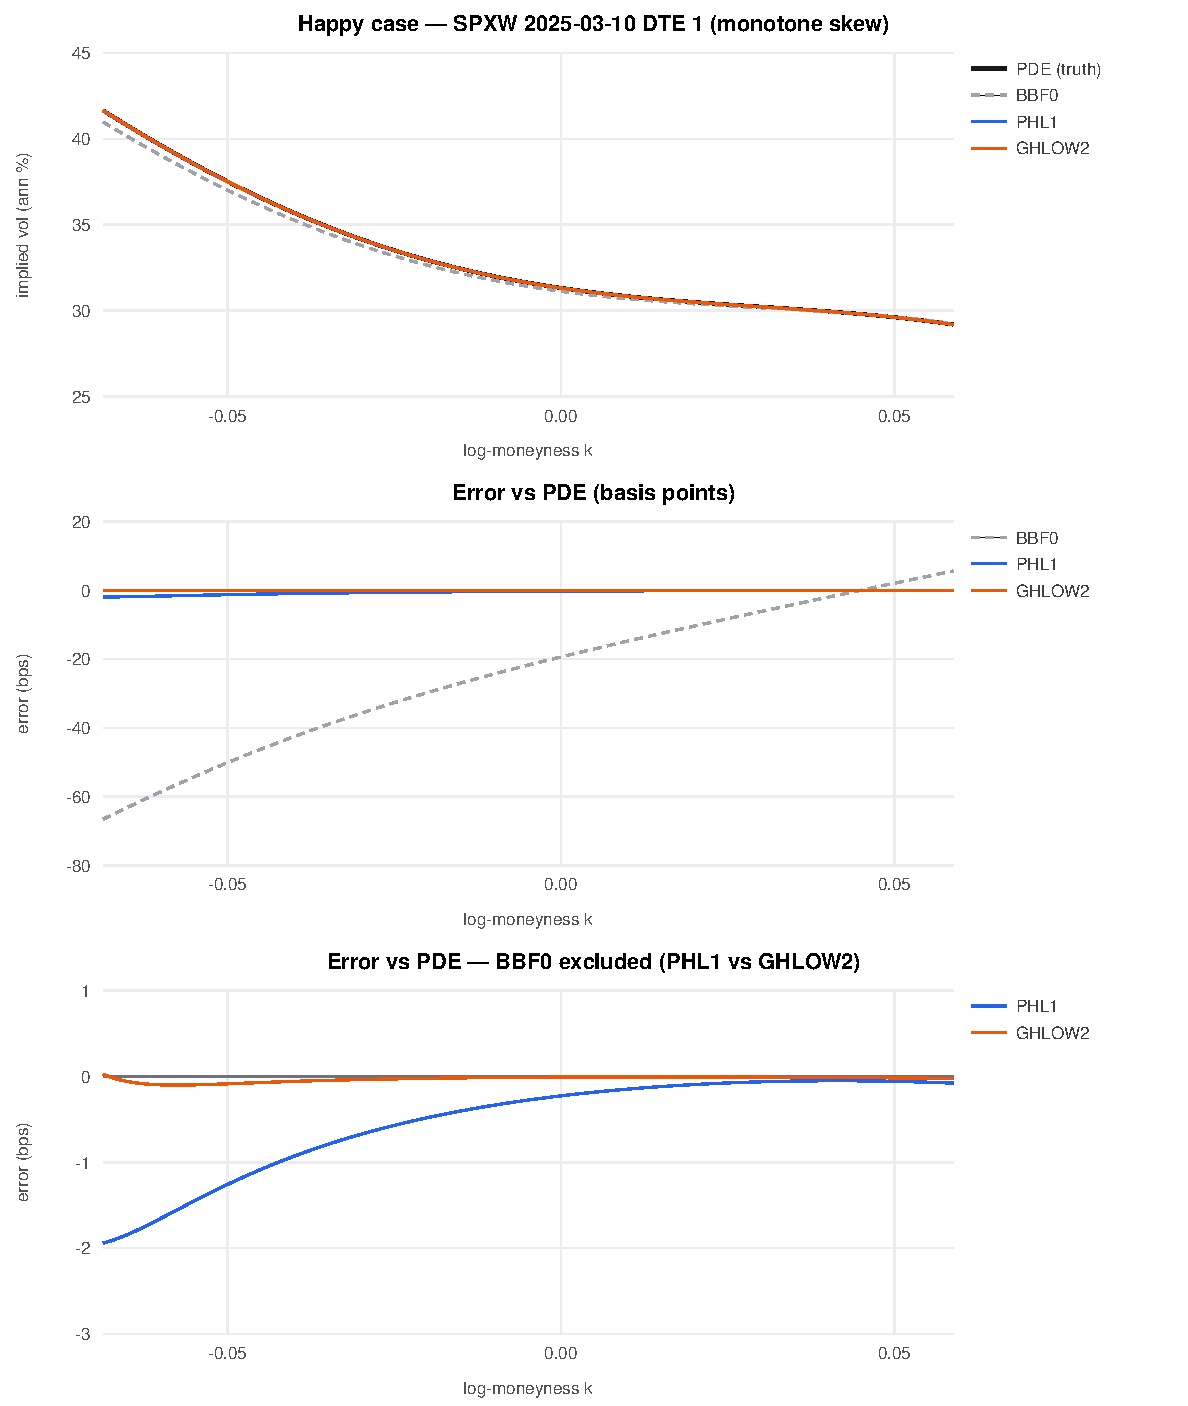
\includegraphics[width=0.78\textwidth]{F1_happy}
\caption{Happy case: smile (top), error vs PDE in bps with BBF0 (middle),
and the same error with BBF0 excluded (bottom) so the PHL1-vs-GHLOW2
comparison is legible.}
\label{fig:happy}
\end{figure}

Figure~\ref{fig:concave}: a concave converted smile (DTE~3).
The approximation remains good where vol is positive; the deep wings, where
the option's time value underflows and implied vol is not recoverable, are
trimmed rather than faked.

\begin{figure}[!htbp]
\centering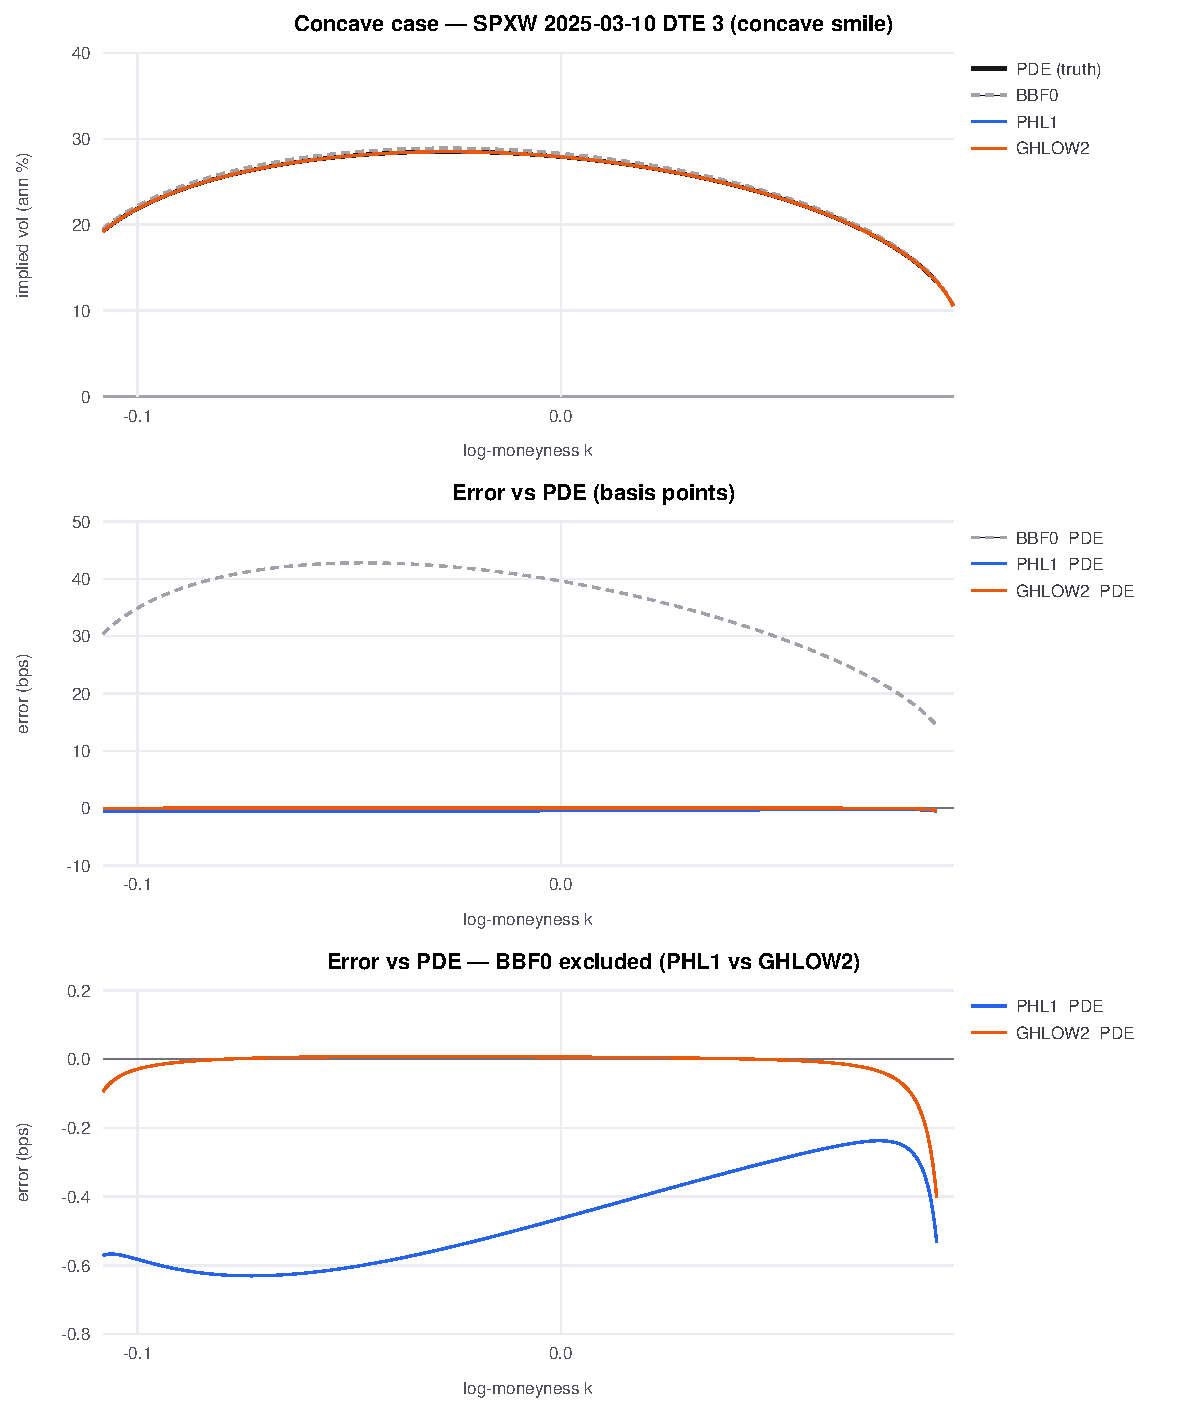
\includegraphics[width=0.78\textwidth]{F2_concave}
\caption{Concave case: the converted smile is concave. Panels as in
Figure~\ref{fig:happy} (smile; error with BBF0; error without BBF0).}
\label{fig:concave}
\end{figure}

Figure~\ref{fig:knot}: the same DTE~1 cubic with a fake ATM knot
($\delta$ the real first-knot jump, moved to $k=0$). PHL1 is visibly
biased near the knot; PHL1c tracks the PDE.

The figure also shows two $T^{2}$-baseline analogues of PHL1c.
\textbf{GHLOW2c} stacks the universal directed kernel
$K_1^{\mathrm{dir}}$ \eqref{eq:K1-dir} on the GHLOW2 baseline:
\begin{equation}
\siv^{\mathrm{GHLOW2c}}(k)=\siv^{\mathrm{GHLOW2}}(k)+R^{(3, 1)}_{1}(k/\sigma, 0).
\label{eq:ghlow2c}
\end{equation}
Equivalently, $\siv^{\mathrm{GHLOW2c}}=\siv^{\mathrm{PHL1c}}+\sigma_2$
in total-vol form. Off the knot it tracks the PDE more tightly than
PHL1c (capturing the smooth $\sigma_2$ term PHL1 omits). It leaves,
however, an analytic value jump at $k=0$ that the universal kernel
cannot reach --- closed by the \emph{extended} directed kernel
introduced below, yielding GHLOW2cc.

\paragraph{The $\sigma_2$ value jump and its repair.}
The universal directed kernel \eqref{eq:K1-dir} subtracts only BBF0's
and $\sigma_1$'s $\delta$-variations from $K_1$. GHLOW2 carries one
more $\delta$-variation, $\sigma_2$'s, and $\sigma_2(0)$ depends on
$\sloc'''(0)=6\gamma$ via the second-order Yoshida coefficient. The
$u_1/u_0$ integrand carries $\sloc'''$ through its first variation, and
the constraint that makes $\sigma_2(0)$ finite leaves a
$\gamma$-linear residual at the next order. Crucially, every Yoshida
ingredient at $k=0$ is algebraic in $(\sigma,\beta,\alpha,\gamma)$ ---
the ATM restriction $w=0$ removes the integrals, just as it removed the
diverging polynomial in $K_1$ --- so the jump is a closed scalar.
The $\gamma$-linear piece of $\sigma_2(0)$ is $\sigma^{3}\beta\gamma/20$,
so $\gamma$ jumping by $\delta$ at the knot produces a GHLOW2 (and
GHLOW2c) value discontinuity
\begin{equation}
\Delta\sigma_2(0)
= \frac{\sigma^{3}\beta\,\delta}{20},
\label{eq:ghlow2-gap}
\end{equation}
which for the SPXW DTE~1 preset is $-0.171$~bps. Subtracting $\sigma_2$'s
$\delta$-variation in addition to BBF0's $x^3/4$ and $\sigma_1$'s $x/4$
gives the \emph{extended} directed kernel:
\begin{equation}
K_1^{\mathrm{ext}}(x,0)
= K_1(x,0)
  - \tfrac{x^3}{4}\Hev(x)
  - \tfrac{x}{4}\Hev(x)
  - \mathrm{clamp}\!\left(
       \frac{\sigma_2(x\sigma;\gamma+\delta)-\sigma_2(x\sigma;\gamma)}{\delta\,\sigma^3};
       \;0,\,\tfrac{\beta}{20}
     \right)\Hev(x).
\label{eq:ghlow2-dir}
\end{equation}
Here $\mathrm{clamp}(z;\,a,b)$ denotes $z$ clipped to the closed
interval between $a$ and $b$ (orientation chosen by their signs;
$\tfrac{\beta}{20}=\Delta\sigma_2(0)/(\delta\sigma^3)$ via
\eqref{eq:ghlow2-gap}).
The first three terms reproduce the universal kernel
\eqref{eq:K1-dir} for $x>0$; the fourth, $(\beta,\alpha,\gamma)$-parametric piece
is the \emph{extension} foreshadowed earlier --- what makes the kernel
\emph{extended}, and what closes the value jump. The extension
lives only on $x>0$ (one-sided perturbation) and the clamp in
\eqref{eq:ghlow2-dir} forces it to zero on the wings. Subtracting
\eqref{eq:K1-dir} from \eqref{eq:ghlow2-dir} and rescaling by
$\delta\,\sigma^{3}$ isolates the extension piece in IV units:
\begin{equation}
R^{(3, 1)}_{2}(k/\sigma, 0) - R^{(3, 1)}_{1}(k/\sigma, 0)
= -\,\mathrm{clamp}\!\left(
   \sigma_2(k;\gamma+\delta) - \sigma_2(k;\gamma);\;
   0,\,\Delta\sigma_2(0)
 \right)\Hev(k).
\label{eq:extension}
\end{equation}
This makes the order content of the extension explicit: it is the
clamped negative of $\sigma_2$'s $\delta$-variation, hence a $T^{2}$
object in the heat-kernel ladder. At $k=0^{+}$ the clamp is inactive
and it takes the value $-\Delta\sigma_2(0)$, exactly cancelling the
GHLOW2c value jump; past the clamp engagement it pins to zero, so on
the wings GHLOW2cc coincides with GHLOW2c. The universal kernel $R_1$
itself remains $T^{3/2}$, so $R_2 = R_1 + (R_2 - R_1)$ is the sum of a
$T^{3/2}$ slope-kink term and a $T^{2}$ value-jump term --- the two
``knot correction'' orders listed for GHLOW2cc in
Table~\ref{tab:summary}.
The fully-corrected GHLOW2 method is then
\begin{equation}
\siv^{\mathrm{GHLOW2cc}}(k)=\siv^{\mathrm{GHLOW2}}(k)+R^{(3, 1)}_{2}(k/\sigma, 0),
\label{eq:ghlow2cc}
\end{equation}
with GHLOW2 again evaluated on the perturbed surface so the cancellation
is exact to first order. The new $\sigma_2$ subtraction is no longer a
universal $x$-only function as the PHL1 kernel's was; it carries the
unperturbed cubic's $(\beta,\alpha,\gamma)$ parametrically, with the
$x=0$ value matching \eqref{eq:ghlow2-gap} exactly. The $w=0$ collapse
that made the bridge integral bounded does \emph{not} extend to the
$\sigma_2$ piece: $\sigma_2$ has a $\xi^{3}/(8 d^{5})$ term with
$d=O(1)$ on the wings, so the raw $\sigma_2$ $\delta$-variation grows
like $k^{3}$. The clamp in \eqref{eq:ghlow2-dir} is what bounds the
construction. At $k=0^{+}$ the raw value equals exactly the cap
$\beta/20$ so the clamp is inactive and the value jump is closed;
past the engagement point ($x\approx 1$ for the SPXW preset) the bare
piece reverses sign and the clamp pins it at $0$, so the extended
kernel collapses back to the universal $K_1^{\mathrm{dir}}$ on the
wings. The clamp is $C^{0}$ but not $C^{1}$ at engagement, outside
the option-meaningful band. The zero-side bound (rather than the
symmetric $\pm|\Delta\sigma_2(0)|$) is what guarantees the wing
collapse.

Figure~\ref{fig:knot} plots all seven curves --- with the asymptotic
order in $T$ at the knot ---
\textbf{PDE} (black, ground truth: Dupire forward equation,
Rannacher-then-Crank--Nicolson);
\textbf{BBF0} (grey dashed, $T^{0}$: inverse harmonic mean, smooth
across the knot since $1/\sloc$ stays $C^{2}$);
\textbf{PHL1} (blue, $T^{1}$: BBF0 $+$ $\sigma_1$, smooth-cubic-accurate
but develops a localised slope kink at $k=0$ because $\sigma_1$'s
derivation assumes $\sloc\in C^{3}$);
\textbf{PHL1c} (red, $T^{1}+T^{3/2}$: PHL1 $+$ universal kernel
$K_1^{\mathrm{dir}}$, repairing the slope kink to first order in
$\delta$);
\textbf{GHLOW2} (teal, $T^{2}$: PHL1 $+$ $\sigma_2$, raising
smooth-cubic accuracy one order but inheriting the PHL1 slope kink and
additionally jumping $-0.171$~bps in $\sigma_2(0)$);
\textbf{GHLOW2c} (amber, $T^{2}+T^{3/2}$: GHLOW2 $+$ universal kernel,
closes the kink but inherits the $\sigma_2$ value jump);
\textbf{GHLOW2cc} (purple, $T^{2}+T^{3/2}$: GHLOW2 $+$ extended kernel,
also closes the value jump)
--- and shows the error ladder for this preset, max $|\mathrm{err}|$ in
bps over the smile band: BBF0 66.6 (off-scale in the middle panel);
PHL1 3.2, capped by a sharp V-shaped slope kink at $k=0$ --- the
signature of $\sigma_1$'s missing $C^3$ assumption; PHL1c 2.0 ---
universal kernel repairs the kink, leaving a broad smooth residual that
is the smooth-cubic $\sigma_2$ piece PHL1c does not move; GHLOW2 3.1
--- still carrying the PHL1 slope kink, now on top of the
$\sigma_2(0)$ value jump; GHLOW2c $0.16$ --- universal kernel closes
the kink, the $\sigma_2$ value jump remains and is visible as a step
from $\sim\!0$ to $-0.15$~bps across $k=0$; GHLOW2cc $0.15$ ---
extended kernel additionally closes that step (continuous at the knot
to numerical precision), strictly improving on GHLOW2c with no
trade-off. The bottom panel, with BBF0 removed, is what makes the PHL1
kink, the PHL1c--GHLOW2 residual swap, the GHLOW2c step, and the
GHLOW2cc collapse legible at all.

Figure~\ref{fig:kernel} plots the two correction pieces separately on
the same knot example. The \emph{universal} piece $R^{(3,1)}_1 =
\delta\,\sigma^{3}\,K_1^{\mathrm{dir}}$ is exactly the gap PHL1c adds
to PHL1 \emph{and} the gap GHLOW2c adds to GHLOW2 (both identical,
sharing the $K_1(0,0)=3\sqrt{2\pi}/128$ peak and decaying on both
sides). The \emph{extension piece} $R^{(3,1)}_2 - R^{(3,1)}_1$ is what
GHLOW2cc adds on top of GHLOW2c: it lives only on $k>0$ (one-sided
perturbation), starts at the closed-form ATM scalar
$|\Delta\sigma_2(0)| = 0.171$~bps that closes the $\sigma_2(0)$ value
jump, and decays to zero on the wings as the clip engages.

\begin{figure}[!htbp]
\centering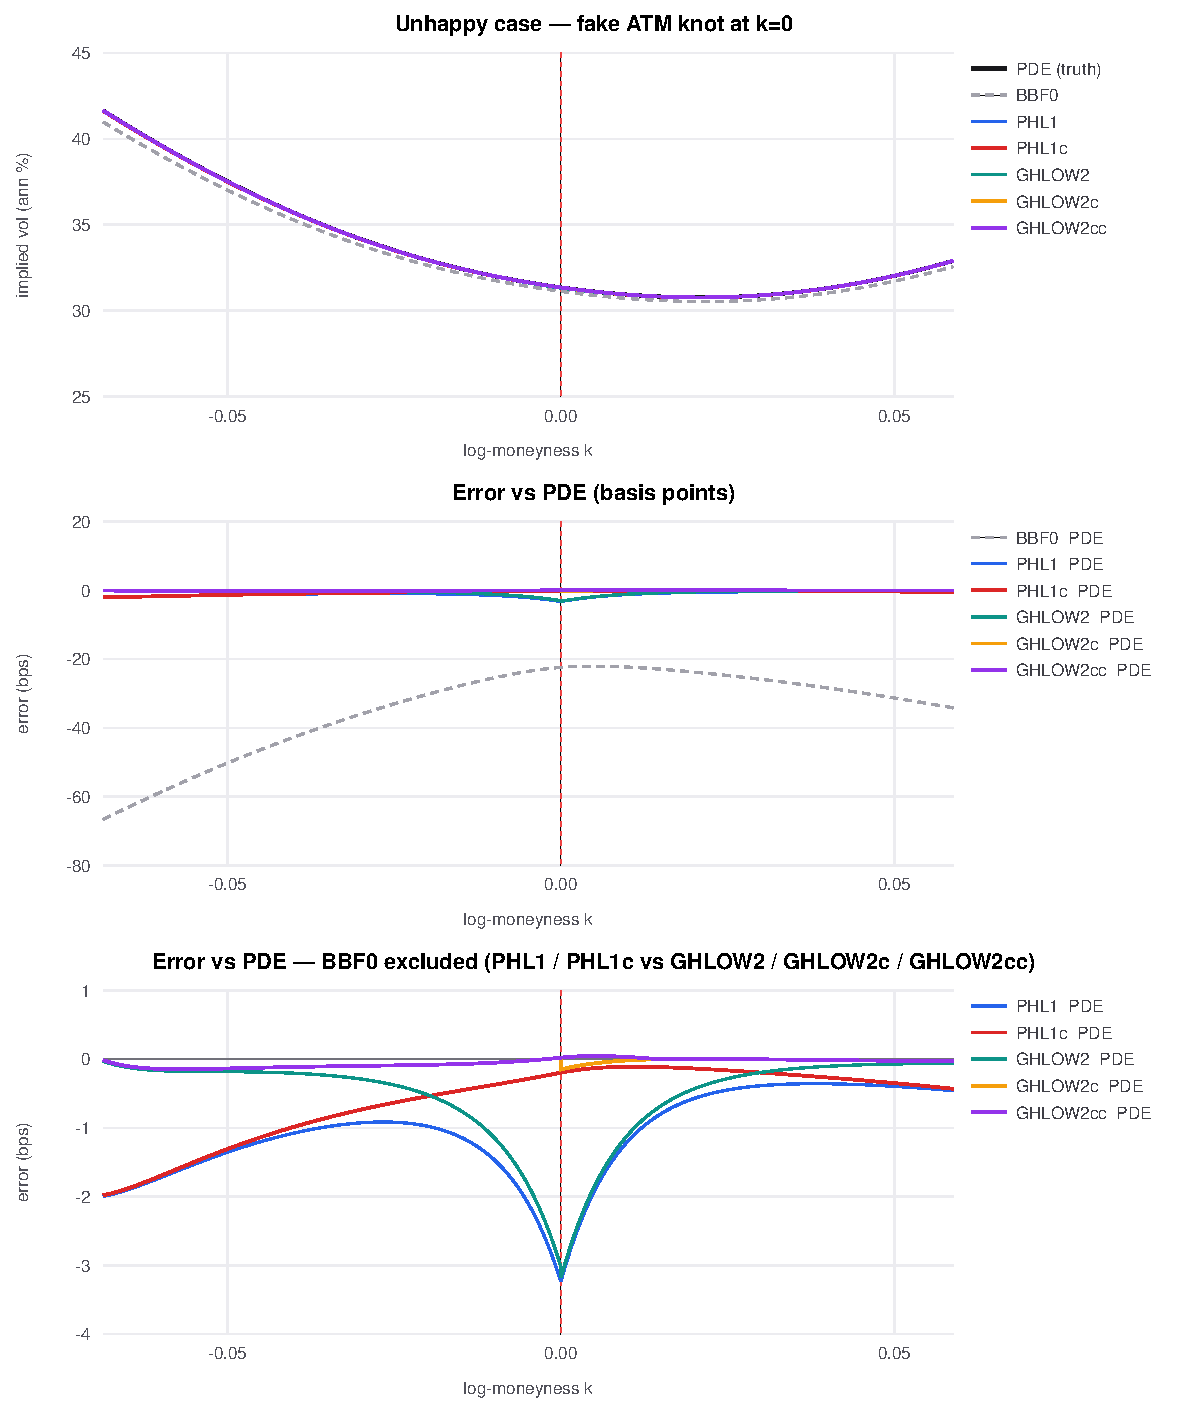
\includegraphics[width=0.78\textwidth]{F3_knot}
\caption{Unhappy case: fake ATM knot at $k=0$. Smile (top); error vs
PDE in bps with BBF0 (middle); same error with BBF0 excluded (bottom)
so the PHL1/PHL1c and GHLOW2/GHLOW2c/GHLOW2cc comparison is legible.
Curves and the error ladder are described in the surrounding text.}
\label{fig:knot}
\end{figure}

\begin{figure}[!htbp]
\centering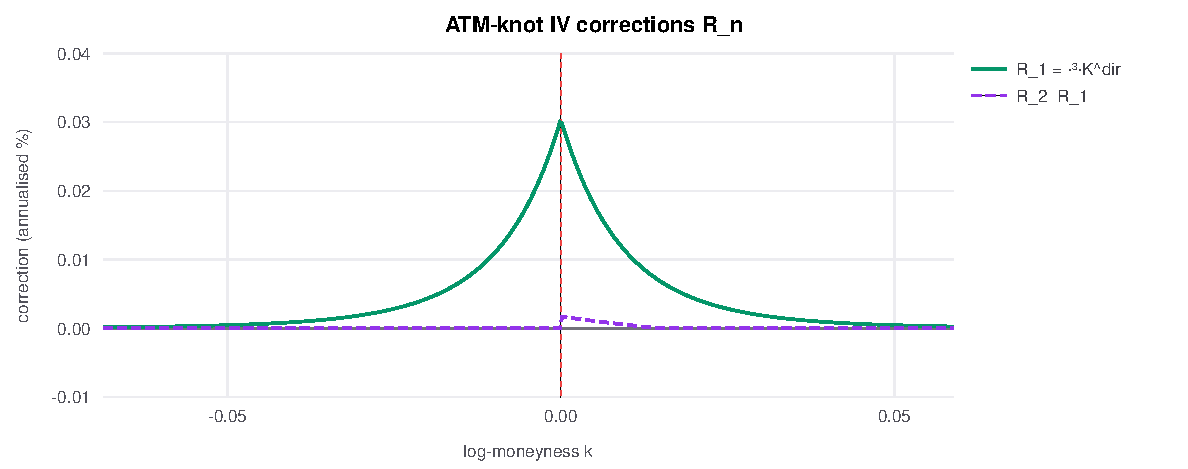
\includegraphics[width=0.72\textwidth]{F4_kernel}
\caption{The two pieces of the ATM-knot correction in annualised \%
for the knot case: universal correction $R^{(3,1)}_1$ (solid green) and
$\sigma_2$ extension piece $R^{(3,1)}_2 - R^{(3,1)}_1$ (dashed purple).
Roles are described in the surrounding text.}
\label{fig:kernel}
\end{figure}

\paragraph{Why the correction is one-sided.}
At every order in the small-$T$ polynomial expansion (BBF0, PHL1,
GHLOW2, $K_1$), the correction for a strike $k$ depends on the
local-vol surface only along the Varadhan-style geodesic between the
forward and the strike, i.e.\ inside $[\min(0,k),\max(0,k)]$. Our
perturbation $\delta k^{3}H(k)$ lives only in $k>0$, so for a strike
$k<0$ the geodesic sits entirely in the untouched region and the
correction is rigorously zero. A Brownian bridge from $0$ to $k<0$
\emph{can} fluctuate into $k>0$, but the probability of that excursion
is $O(\exp(-c/T))$ --- non-perturbative, below every polynomial-in-$T$
term in the expansion. The Dupire PDE captures the exponentially small
cross-side leakage; the closed-form maps do not, by design.

\section{Conclusion}

BBF calibrates any smile but gives no arbitrage guarantee; PHL1 supplies
that guarantee but a single smooth cubic through it is too rigid to span
the smiles BBF can reach. The obvious way to regain flexibility --- a knot
--- was blocked by one defect: a piecewise cubic is only $C^2$ at a knot
while PHL1's $\sigma_1$ expansion assumes $C^3$, so PHL1 develops a
localised residual at the knot strike (BBF, a harmonic-mean integral, is
insensitive to it and has no knot-specific error). This paper removed that
single defect for a knot pinned at-the-money, in closed form: the
first-order Duhamel kernel $K_1(x,0)$, a one-dimensional bridge
integral with peak $3\sqrt{2\pi}/128$ and no fitted constants. After subtracting the
variation PHL1 already captures, the residual decays on both sides
and adds directly to PHL1. On parameters calibrated from real SPXW
surfaces PHL1c tracks the Dupire PDE where PHL1 alone is biased, and
the correction is inert on smooth smiles.

The consequence is practical, not just numerical: ``piecewise-cubic with
an at-the-money knot, mapped through PHL1'' is now a usable surface
parametrisation --- it keeps PHL1's arbitrage reassurance while recovering
the calibration flexibility a single smooth cubic lacks, the knot adding
shape freedom exactly where the smile is most curved. The at-the-money
restriction is essential, not cosmetic: off-the-money the same
construction leaves an unbounded polynomial requiring an ad-hoc
truncation; $w=0$ removes that term and fixes the peak by a
Beta-function moment. The peak $3\sqrt{2\pi}/128$ is the $C^{2}$
companion, in log-normal Black IV, to the $C^{0}$ normal-IV constant
$\tfrac{1}{16}\sqrt{\pi/2}$ of Costeanu and Pirjol --- adjacent slots
of the same Duhamel-perturbation table they began. The same $w=0$
collapse extends naturally to the $T^{2}$ baseline: stacking the same
universal kernel on GHLOW2 gives GHLOW2c, which inherits the
smooth-cubic $\sigma_2$ accuracy off the knot but still carries a
$\gamma$-linear value jump in $\sigma_2$ given in closed form by
\eqref{eq:ghlow2-gap}; subtracting $\sigma_2$'s $\delta$-variation in
\eqref{eq:ghlow2-dir} closes that jump as well, yielding the
value-continuous GHLOW2cc. The remaining natural extension is the
$w\neq0$ case --- moving the knot off the forward --- which is more
involved because the bounded-polynomial collapse used here disappears.

\section{Reproducibility}

All numbers and figures are produced by the open TypeScript core in the
companion repository, cross-checked against a committed numerical fixture
to $10^{-6}$ (closed forms) and $10^{-9}$ (the kernel), and against the
Dupire forward PDE on the knot-case model within tolerance. The figures
are deterministic: regenerating them and diffing reproduces this paper
exactly.

\paragraph{Credits.} Market data for the calibrated example smiles:
ThetaData.

\bibliographystyle{plainnat}
\bibliography{refs}

\end{document}
